%%%%%%%%%%%%%%%%%%%%%%%%%%%%%%%%%%%%%%%%%%%%%%%%%%%%%%%%%%%%%%%%%%%%%%
%%  Copyright by Wenliang Du.                                       %%
%%  This work is licensed under the Creative Commons                %%
%%  Attribution-NonCommercial-ShareAlike 4.0 International License. %%
%%  To view a copy of this license, visit                           %%
%%  http://creativecommons.org/licenses/by-nc-sa/4.0/.              %%
%%%%%%%%%%%%%%%%%%%%%%%%%%%%%%%%%%%%%%%%%%%%%%%%%%%%%%%%%%%%%%%%%%%%%%

\documentclass[11pt]{article}

\usepackage[most]{tcolorbox}
\usepackage{times}
\usepackage{epsf}
\usepackage{epsfig}
\usepackage{amsmath, alltt, amssymb, xspace}
\usepackage{wrapfig}
\usepackage{fancyhdr}
\usepackage{url}
\usepackage{verbatim}
\usepackage{fancyvrb}
\usepackage{adjustbox}
\usepackage{listings}
\usepackage{color}
\usepackage{subfigure}
\usepackage{cite}
\usepackage{sidecap}
\usepackage{pifont}
\usepackage{mdframed}
\usepackage{textcomp}
\usepackage{enumitem}


% Horizontal alignment
\topmargin      -0.50in  % distance to headers
\oddsidemargin  0.0in
\evensidemargin 0.0in
\textwidth      6.5in
\textheight     8.9in 

\newcommand{\todo}[1]{
\vspace{0.1in}
\fbox{\parbox{6in}{TODO: #1}}
\vspace{0.1in}
}


\newcommand{\unix}{{\tt Unix}\xspace}
\newcommand{\linux}{{\tt Linux}\xspace}
\newcommand{\minix}{{\tt Minix}\xspace}
\newcommand{\ubuntu}{{\tt Ubuntu}\xspace}
\newcommand{\setuid}{{\tt Set-UID}\xspace}
\newcommand{\openssl} {\texttt{openssl}}


\pagestyle{fancy}
\lhead{\bfseries SEED Labs}
\chead{}
\rhead{\small \thepage}
\lfoot{}
\cfoot{}
\rfoot{}


\definecolor{dkgreen}{rgb}{0,0.6,0}
\definecolor{gray}{rgb}{0.5,0.5,0.5}
\definecolor{mauve}{rgb}{0.58,0,0.82}
\definecolor{lightgray}{gray}{0.90}


\lstset{%
  frame=none,
  language=,
  backgroundcolor=\color{lightgray},
  aboveskip=3mm,
  belowskip=3mm,
  showstringspaces=false,
%  columns=flexible,
  basicstyle={\small\ttfamily},
  numbers=none,
  numberstyle=\tiny\color{gray},
  keywordstyle=\color{blue},
  commentstyle=\color{dkgreen},
  stringstyle=\color{mauve},
  breaklines=true,
  breakatwhitespace=true,
  tabsize=3,
  columns=fullflexible,
  keepspaces=true,
  escapeinside={(*@}{@*)}
}

\newcommand{\newnote}[1]{
\vspace{0.1in}
\noindent
\fbox{\parbox{1.0\textwidth}{\textbf{Note:} #1}}
%\vspace{0.1in}
}


%% Submission
\newcommand{\seedsubmission}{You need to submit a detailed lab report, with screenshots,
to describe what you have done and what you have observed.
You also need to provide explanation
to the observations that are interesting or surprising.
Please also list the important code snippets followed by
explanation. Simply attaching code without any explanation will not
receive credits.}

%% Book
\newcommand{\seedbook}{\textit{Computer \& Internet Security: A Hands-on Approach}, 2nd
Edition, by Wenliang Du. See details at \url{https://www.handsonsecurity.net}.}

%% Videos
\newcommand{\seedisvideo}{\textit{Internet Security: A Hands-on Approach},
by Wenliang Du. See details at \url{https://www.handsonsecurity.net/video.html}.}

\newcommand{\seedcsvideo}{\textit{Computer Security: A Hands-on Approach},
by Wenliang Du. See details at \url{https://www.handsonsecurity.net/video.html}.}

%% Lab Environment
\newcommand{\seedenvironment}{This lab has been tested on our pre-built
Ubuntu 16.04 VM, which can be downloaded from the SEED website. }

\newcommand{\seedenvironmentA}{This lab has been tested on our pre-built
Ubuntu 16.04 VM, which can be downloaded from the SEED website. }

\newcommand{\seedenvironmentB}{This lab has been tested on our pre-built
Ubuntu 20.04 VM, which can be downloaded from the SEED website. }

\newcommand{\seedenvironmentAB}{This lab has been tested on our pre-built
Ubuntu 16.04 and 20.04 VMs, which can be downloaded from the SEED website. }

\newcommand{\nodependency}{Since we use containers to set up the lab environment, 
this lab does not depend too much on our SEED VM. You can do this lab
using other VMs or physical machines. }







\newcommand{\seedlabcopyright}[1]{
\vspace{0.1in}
\fbox{\parbox{6in}{\small Copyright \copyright\ {#1}\ \ by Wenliang Du.\\
      This work is licensed under a Creative Commons
      Attribution-NonCommercial-ShareAlike 4.0 International License.
      If you remix, transform, or build upon the material, 
      this copyright notice must be left intact, or reproduced in a way that is reasonable to
      the medium in which the work is being re-published.}}
\vspace{0.1in}
}





\newcommand{\rebindingFigs}{./Figs}

\lhead{\bfseries SEED Labs -- DNS Rebinding Attack Lab}


\begin{document}

\begin{center}
{\LARGE DNS Rebinding Attack Lab}

\vspace{0.05in}
Updated on February 10, 2020
\end{center}

\seedlabcopyright{2019}


\newcounter{task}
\setcounter{task}{1}
\newcommand{\tasks} {\bf {\noindent (\arabic{task})} \addtocounter{task}{1} \,}



% *******************************************
% SECTION
% ******************************************* 
\section{Introduction}


The objective of this lab is two-fold: (1) demonstrate how 
the DNS rebinding attack works, and (2) help students gain
the first-hand experience on how to use the DNS rebinding
technique to attack IoT devices. In the setup, we have a simulated IoT device, 
which can be controlled through
a web interface (this is typical for many IoT devices). Many IoT devices do not have 
a strong protection mechanism, if attackers can directly interact with them, they can
easily compromise these devices. 


The IoT device simulated in this lab is a thermostat, 
which controls the room temperature. 
To successfully set the temperature, the client needs to be able to interact with the
IoT server. Since the IoT device is behind the firewall, outside machines
cannot interact with the IoT device, and will therefore not be able to 
control the thermostat. To defeat the firewall protection, the attacking code must get into the 
internal network first. This is not difficult. Any time when a user from 
the internal network visits the attacker's website, the attacker's code (JavaScript
code) actually runs from the user's browser, and therefore runs inside the 
protected internal network. However, due to the sandbox protection implemented 
by browsers, the attacker's code still cannot interact with the IoT device, even though it 
is now inside the internal network. 


The objective of this lab is to use the DNS rebinding attack to 
circumvent the sandbox protection, so
the JavaScript code from the attacker can successfully get the 
essential information from the IoT device and then 
use the information to set the temperature 
of the thermostat to a dangerously high value. This lab covers the
following topics:

\begin{itemize}[noitemsep]
\item DNS server setup
\item DNS rebinding attack
\item Attacks on IoT devices
\item Same Origin Policy
\end{itemize}


\paragraph{Readings and videos.}
Detailed coverage of the DNS protocol and attacks can be found in the following:

\begin{itemize}
\item Chapter 18 of the SEED Book, \seedbook
\item Section 7 of the SEED Lecture, \seedisvideo
\end{itemize}


\paragraph{Lab environment.} \seedenvironment



\vspace{0.2in}
\noindent
\fbox{\parbox{\textwidth}{
\noindent
\textbf{Customization.} 
In this lab description, we use the domain \texttt{attacker32.com} to refer to the 
domain controlled by the attacker. When students do this lab, they are not allowed 
to use this domain name; instead, they should use a name that includes 
their last names (the domain name is only used internally inside the VMs, so it does not 
matter whether the name is owned by others or not). 
The purpose of this requirement is to differentiate student's work.
}}





% *******************************************
% SECTION
% ******************************************* 
\section{Background: IoT}

Our attack target is an IoT device behind the firewall. We cannot directly
access this IoT device from outside. Our goal is to get an inside
user to run our JavaScript code, so we can use
the DNS rebinding attack to interact with the IoT device.


Many IoT devices have a simple built-in web server, so users can
interact with these devices via web APIs. Typically, these IoT
devices are protected by a firewall, they cannot be accessed directly
from outside. Due to this type of protection,  many IoT devices do not
implement a strong authentication mechanism. If attackers can find ways
to interact with them, they can easily compromise its security.

We emulate such a vulnerable IoT device using 
a simple web server, which serves
two APIs: \texttt{password} and \texttt{temperature}.
The IoT device can set the room temperature. To do that,
we need to send out an HTTP request to the server's
\texttt{temperature} API; the request should include
two pieces of data: the target temperature value and a
password.  The password is a secret that changes
periodically, but it can be fetched using
the \texttt{password} API. Therefore, to successfully
set the temperature, users needs to
first get the password, and then attach the password
in the \texttt{temperature} API.

The password is not meant for the authentication purpose; it is used to defeat the Cross-Site
Request Forgery (CSRF) attack. Without this protection, a simple CSRF attack is sufficient;
there is no need to use the more sophisticated DNS rebinding attack.
For the sake of simplicity, we hardcoded the
password; in real systems, the password will be re-generated periodically.




% *******************************************
% SECTION
% ******************************************* 
\section{Lab Environment Setup}

\begin{figure}[htb]
\centering
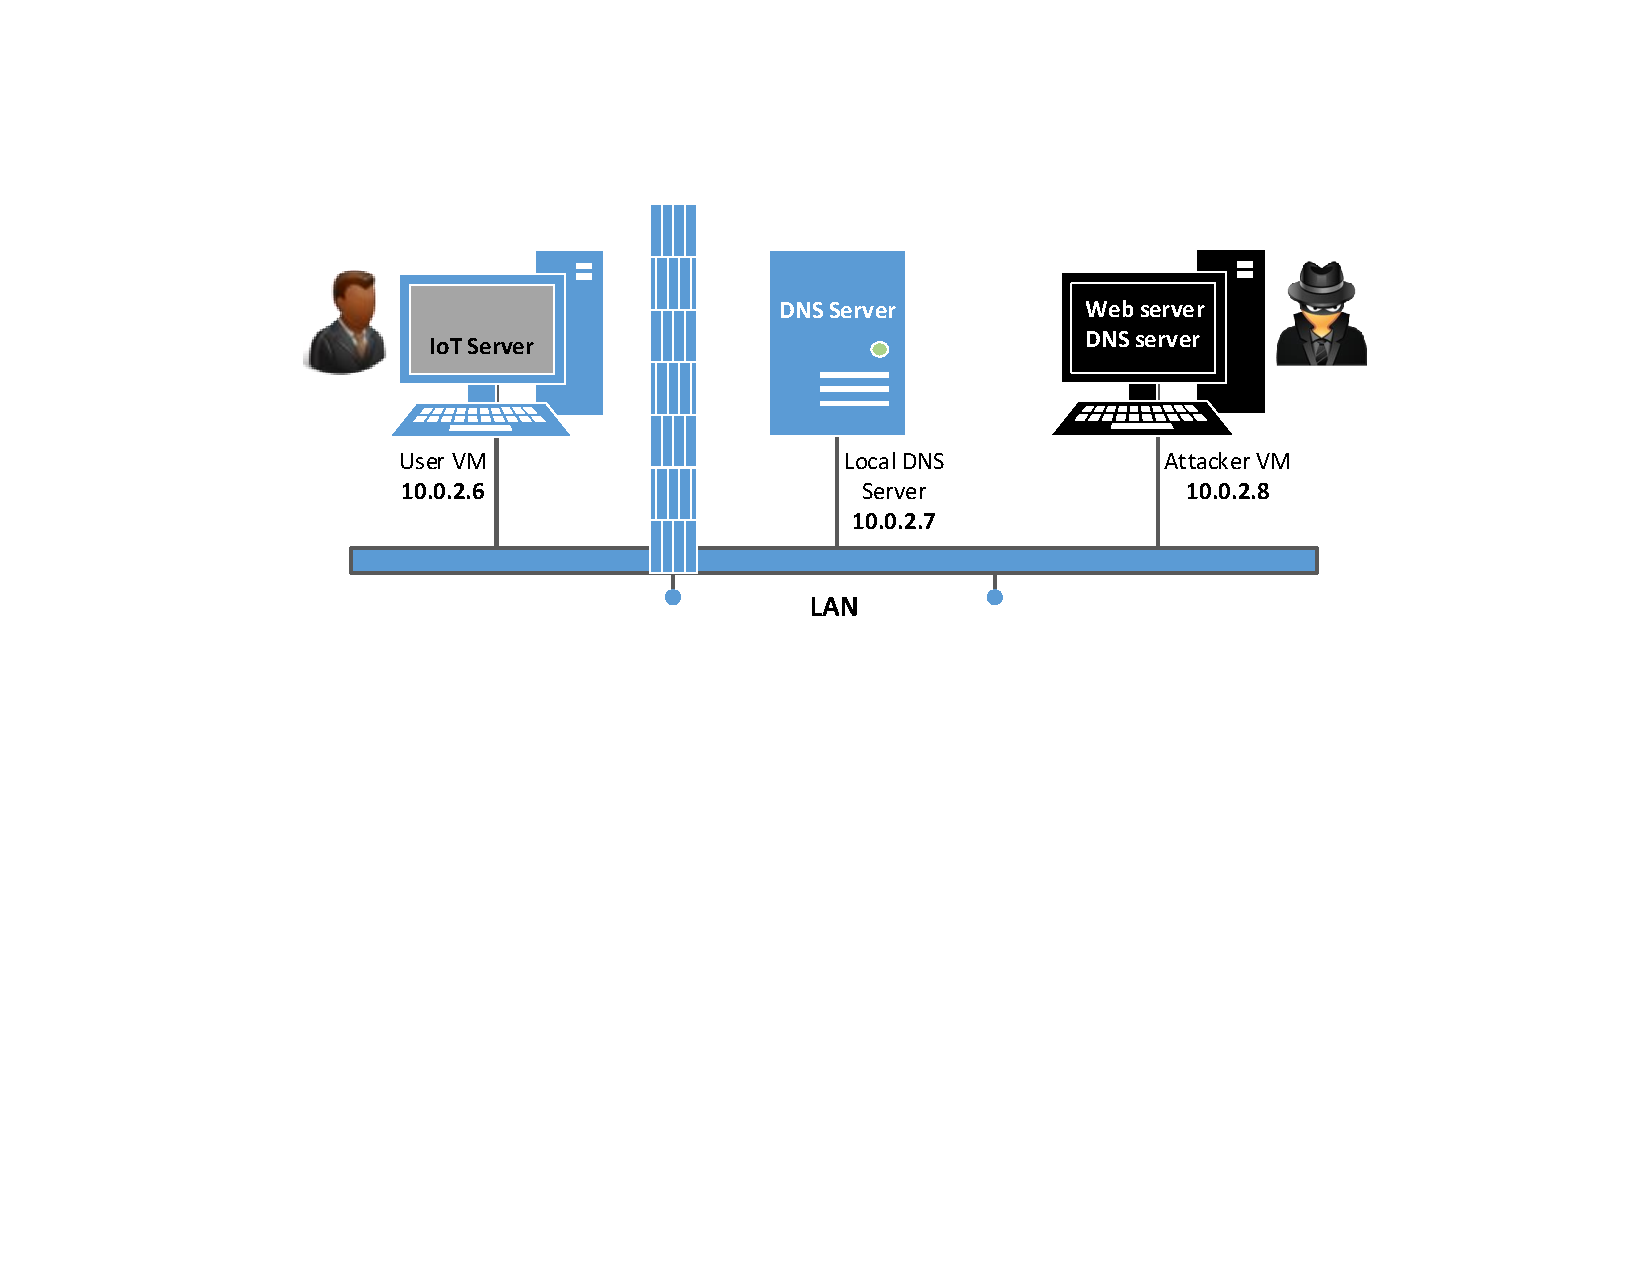
\includegraphics[width=0.9\textwidth]{\rebindingFigs/environment_setup_rebind.pdf}
\caption{Environment setup for the experiment}
\label{dns:fig:rebind_environment}
\end{figure}


In this lab, we will use three machines (VMs), which will be called 
User VM, Local DNS Server, and Attacker VM. For the sake of simplicity,
we place these VMs on the same network using the NAT Network adaptor in VirtualBox. In the 
real world, they are not on the same network.
We also assume that IoT device, which is running on the user VM, 
is behind the firewall, so the attacker VM cannot directly
access the IoT device. 
The setup of this lab is quite complicated, as we need to 
configure three VMs and run multiple servers on them, including 
an IoT web server (on User VM), a web server and a DNS server (on Attacker
VM), and a DNS server (on the Local DNS server). 
We break down the setup into 5 tasks. 


In the rest of the document, we assume that the User VM's IP address is
{\tt 10.0.2.6}, the local DNS Server's IP is {\tt 10.0.2.7} and the Attacker
VM's IP is {\tt 10.0.2.8}. The lab environment setup is illustrated
in Figure~\ref{dns:fig:rebind_environment}. 



% -------------------------------------------
% SUBSECTION
% ------------------------------------------- 
\subsection{Task 1: Configure the User VM}

\paragraph{Step 1. Reduce Firefox's DNS caching time.}
To reduce load on DNS servers and to speed up response time, Firefox browser caches DNS
results.  By default, the cache's expiration time is 60 seconds. That means that our DNS
rebinding attack needs to wait for at least 60 seconds. To make our life easier, we reduce
the time to 10 seconds or less. Type \texttt{about:config} in the URL field.
After clicking through a warning page, we will see a list of preference names and their values.
Search for \texttt{dnsCache}, find the following entry and change its value:

\begin{lstlisting}
(*@\textbf{network.dnsCacheExpiration}@*):  change its value to 10 (default is 60)
\end{lstlisting}

After making the change, we should exit from the Firefox browser, and restart it; otherwise the
change will not take effect.



\paragraph{Step 2. Change \texttt{/etc/hosts}.}
We need to add the following entry to the \texttt{/etc/hosts} file. 
We will use \texttt{www.seeedIoT32.com} as the name for the 
IoT web server. This server can run on a different VM, but for the 
sake of simplicity, we run the IoT server on the User VM (assuming 
its IP address is \texttt{10.0.2.6}): 


\begin{lstlisting}
10.0.2.6   www.seedIoT32.com
\end{lstlisting}
 


\paragraph{Step 3. Local DNS Server.}
We need to configure the User VM to use a particular local DNS server. This is achieved by
setting the local DNS server as the first \texttt{nameserver} entry in the resolver
configuration file (\texttt{/etc/resolv.conf}). 
One challenge is that the provided VM uses the
Dynamic Host Configuration Protocol (DHCP) to obtain network configuration parameters, such as
IP address, local DNS server, etc. DHCP clients will overwrite the \texttt{/etc/resolv.conf}
file with the information provided by the DHCP server.

One way to get our information into \texttt{/etc/resolv.conf} without worrying about
the DHCP is to add the following entry to the \path{/etc/resolvconf/resolv.conf.d/head}
file (assuming that \texttt{10.0.2.7} is the IP address of the local DNS server):

\begin{lstlisting}
nameserver 10.0.2.7
\end{lstlisting}

The content of the head file will be prepended to the dynamically generated resolver
configuration file. Normally, this is just a comment line (the comment in
\texttt{/etc/resolv.conf} comes from this head file). After making the change,
we need to run the following command for the change to take effect: 

\begin{lstlisting}
$ sudo resolvconf -u
\end{lstlisting}


%----------------------------
\paragraph{Step 4. Testing.}
After configuring the user VM, use the \texttt{dig} command
to get an IP address from a hostname of your choice. From the response, please provide
evidences to show that the response is indeed from your server. If you cannot find the
evidence, your setup is not successful.



% -------------------------------------------
% SUBSECTION
% ------------------------------------------- 
\subsection{Task 2: Start the IoT server on the User VM}

In this task, we will start the IoT server on the User VM. 
Through the web server, users can communicate with the 
IoT device.


%-----------
\paragraph{Step 1. Install Flask.}
We used the \texttt{Flask} web framework to develop the
IoT server. In the current version of the SEED VM, \texttt{Flask} 
has not been installed, so we need to install it first.
Use the following command to install \texttt{Flask}.

\begin{lstlisting}
$ sudo pip3 install Flask==1.1.1
\end{lstlisting}


%-----------
\paragraph{Step 2. Start the IoT server.}
The IoT server code is included in \texttt{user\_vm.zip}, which 
can be downloaded from the lab's website. After unzipping the file,
enter the \texttt{user\_vm} folder, and start the IoT server 
by either running the prepared script \texttt{start\_iot.sh} 
or running \texttt{"flask run"} directly. It should be noted 
that we use port \texttt{8080} for the IoT server (this port number is 
hard-coded in the lab setup; changing it to a different number
will break the lab setup).


\begin{lstlisting}
$ unzip user_vm.zip          # Unzip the file
$ cd user_vm                 # Go to the user_vm folder
$ FLASK_APP=rebind_iot flask run --host 0.0.0.0 --port 8080
\end{lstlisting}
 

%-----------
\paragraph{Step 3. Testing the IoT server.}
To test the IoT server, point the browser to the following URL on the 
User VM. If everything is setup correctly, we should be able to see 
a thermostat. We can also change the temperature setting by dragging the 
sliding bar. Please provide a screenshot in your lab report. 

\begin{lstlisting}
http://www.seedIoT32.com:8080
\end{lstlisting}



% -------------------------------------------
% SUBSECTION
% ------------------------------------------- 
\subsection{Task 3: Start the attack web server on the Attacker VM}

In this lab, the IoT device is only accessible from behind the firewall, i.e., 
only from the User VM in the lab setup. A typical way to get our 
malicious code onto the User VM is to get the user to visit 
our website, so the JavaScript code placed on our web pages 
can get into the User VM. In this task, we will start 
a web server to host such web pages. 

%-----------
\paragraph{Step 1. Install Flask}
Our malicious web server is also developed based on the 
\texttt{Flask} web framework, so we need to 
install it first on the Attacker VM. 


\begin{lstlisting}
$ sudo pip3 install Flask==1.1.1
\end{lstlisting}


%-----------
\paragraph{Step 2. Start the attacker's web server}
The attacker's server code is included in \texttt{attacker\_vm.zip}, which
can be downloaded from the lab's website. After unzipping the file,
enter the \texttt{attacker\_vm} folder, and start the web server by
running the prepared script \texttt{start\_webserver.sh} or running
\texttt{"flask run"} directly. 



\begin{lstlisting}
$ unzip attacker_vm.zip      # unzip the file
$ cd attacker_vm             # Go to the attacker_vm folder
$ FLASK_APP=rebind_malware flask run --host 0.0.0.0 --port 8080
\end{lstlisting}



%-----------
\paragraph{Step 3. Testing the Attacker's web server.}
Point the browser to the following URL on the Attacker VM, and you should 
be able to see the attacker's website. 
Please provide a screenshot in your lab report. 


\begin{lstlisting}
http://localhost:8080
\end{lstlisting}


% -------------------------------------------
% SUBSECTION
% ------------------------------------------- 
\subsection{Task 4: Configure the DNS server on the Attacker VM}

The Attacker VM also serves as the nameserver for the \texttt{attacker32.com}
domain. The BIND9 server is already running on the Attacker VM, and 
we need to prepare a zone file for it. A sample 
zone file is included in the \texttt{attacker\_vm} folder.  Students should 
change the zone file accordingly, and copy it into the \texttt{/etc/bind} 
folder. The following shows the content of the sample zone file. The first 
entry is the default Time-To-Live (\texttt{TTL}) value (seconds) 
for the response, specifying how long the response can stay in
the DNS cache. In later tasks, this value may
need to be modified. 

\begin{lstlisting}
$TTL 10000
@       IN      SOA   ns.attacker32.com. admin.attacker32.com. (
                2008111001
                8H
                2H
                4W
                1D)

@       IN      NS    ns.attacker32.com.

@       IN      A     10.0.2.8
www     IN      A     10.0.2.8
ns      IN      A     10.0.2.8
*       IN      A     10.0.2.8
\end{lstlisting}
 

You need to add the following zone entry to \texttt{/etc/bind/named.conf},
so the above zone file will be used by the BIND9 server. 

\begin{lstlisting}
zone "attacker32.com" {
        type master;
        file "/etc/bind/attacker32.com.zone";
};
\end{lstlisting}
 

After making changes to the \texttt{named.conf} file, we need to 
restart the BIND9 server using the following command. 

\begin{lstlisting}
$ sudo service bind9 restart
\end{lstlisting}
 

\paragraph{Testing.} If everything is set up correctly, we can
try the following \texttt{dig} command to see whether the response we get 
is the same as what we put in the zone file. Please include your 
observation (screenshots) in the lab report. 

\begin{lstlisting}
// Test DNS server (change 10.0.2.8 to the Attacker VM's IP)
$ dig @10.0.2.8 www.attacker32.com
\end{lstlisting}



% -------------------------------------------
% SUBSECTION
% ------------------------------------------- 
\subsection{Task 5: Configure the Local DNS Server}


In the previous task, we have set up the nameserver for the 
\texttt{attacker32.com} domain (or the customized name chosen
by students) on the attacker VM. In order for others to find
this nameserver, we need to register 
our nameserver with the \texttt{.com} nameserver, so 
an \texttt{NS} record is added to its database. Without this step,
DNS requests from others will not be able to reach our nameserver. 


To do this, not only do we need to purchase the domain, we also need to 
run our nameserver on a public computer, not a VM inside 
a private network (our VM is not 
accessible from the outside). While all of these are doable, it 
increases the cost and complexity of the lab setup. We 
use a much simpler approach to simulate the real-world
scenario. 

On the Local DNS server, we set up a forward record for 
the \texttt{attacker32.com} domain, so  
whenever the local DNS server receives a DNS query for hosts inside this domain, 
it will simply send the DNS query to the IP 
address specified in the forward record, instead of going to the root server
and then the \texttt{.com} server to find out where the nameserver for the 
\texttt{attacker32.com} domain is.  


To add such 
a record to the Local DNS server, 
we need to add the following lines 
to \path{/etc/bind/named.conf} (it should be noted that students should use 
their own customized domain name, instead of using \texttt{attacker32.com}).

\begin{lstlisting}
zone "attacker32.com" {
    type forward;
    forwarders { 10.0.2.8; };
};
\end{lstlisting}

If you copy and paste the above lines from the PDF file, be aware that the 
quotation symbols may not be correct, which may introduce
errors to the configuration file. It is better to delete them, and 
retype the quotation symbols. After configuring BIND9, 
we need to restart the DNS server using the following command: 


\begin{lstlisting}
$ sudo service bind9 restart
\end{lstlisting}

%Check the BIND9's log file at \texttt{/var/log/syslog} to
%see whether there is any error message. 


\paragraph{Testing.}
If we have done Tasks 1-5 correctly, when we run the following 
\texttt{dig} command on the User VM to find out the IP address of 
any host inside the \texttt{attacker32.com} domain, we should  
get the value that is put inside the \texttt{attacker32.com}'s 
zone file on the attacker VM. 


\begin{lstlisting}
$ dig xyz.attacker32.com
\end{lstlisting}
 


Please include your observations (screenshots) 
in the lab report. 
If you do not get this IP address, you may have done 
something wrong in one of the steps. You should 
fix it before proceeding to the next task. 




% *******************************************
% SECTION
% ******************************************* 
\section{Launch the Attack on the IoT Device}

We are ready to launch the attack on the IoT device. To help students 
understand how the attack works, we break down
the attack into several incremental steps. 

\subsection{Task 6. Understanding the Same-Origin Policy Protection}

In this task, we will do some experiment to understand the 
same-origin policy protection implemented on browsers. On the User VM,
we will browse the following three URLs. It is better to show these three pages on three
different Firefox windows (instead of on three different tabs), so they are all visible. 


\begin{lstlisting}
URL 1:  http://www.seedIoT32.com:8080
URL 2:  http://www.seedIoT32.com:8080/change
URL 3:  http://www.attacker32.com:8080/change
\end{lstlisting}

 
The first page lets us see the current temperature setting of the thermostat (see
Figure~\ref{rebinding:fig:webpages}.a); it fetches
the temperature value from the IoT server once every second. We should keep this page always
visible, so we can see the temperature setting on the thermostat. 
The second and third pages
are identical (see Figure~\ref{rebinding:fig:webpages}.b), 
except that one comes from the IoT server, and the other comes from
the attacker's server. When we click the button on both pages, 
a request will be sent out to the IoT server to set its temperature. 
we are supposed to raise the thermostat's temperature 
to \texttt{99} Celsius.  


\begin{figure}[htb]
\begin{center}
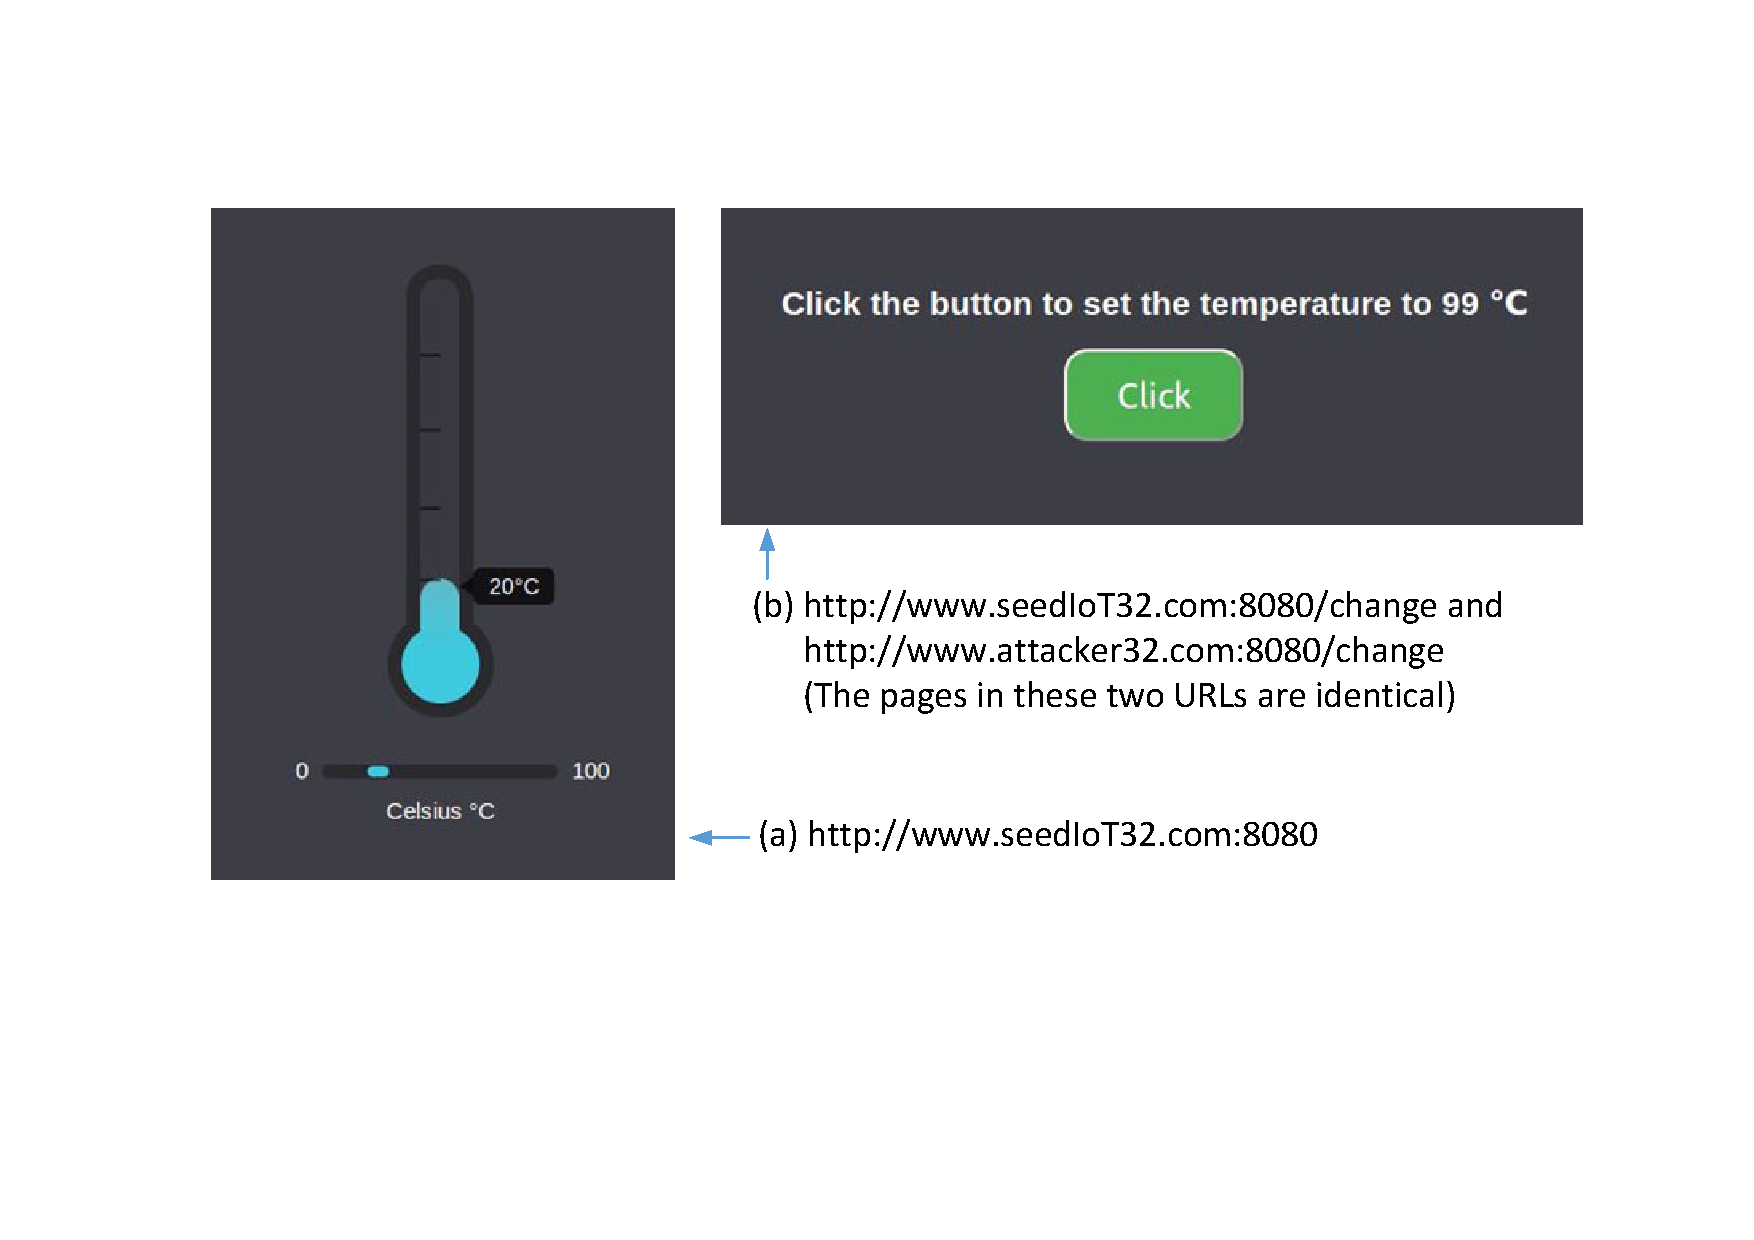
\includegraphics[width=0.8\textwidth]{\rebindingFigs/iot_webpages.pdf}
\end{center}
\caption{The web pages from the three URLs}
\label{rebinding:fig:webpages}
\end{figure}
 

Click the button on the second and third pages, and describe your observation. Which page
can successfully set the thermostat's temperature? Please explain why. 
To find the reason, click the following menu sequence from Firefox. A console window will appear,
which displays error messages if any. Hint: the reason is related to the same-origin policy 
enforced by browsers. Please explain why this policy causes one of the pages to fail.
 
\begin{lstlisting}
Tools -> Web Developer -> Web Console
\end{lstlisting}
  



% -------------------------------------------
% SUBSECTION
% ------------------------------------------- 
\subsection{Task 7. Defeat the Same-Origin Policy Protection}


From the previous task, it seems impossible to
set the thermostat's temperature from the attacker's
page, due to the browser's   
same-origin policy protection.  The objective of this task
is to defeat such a protection, so we can set the 
temperature from this page. 


The main idea for defeating the same origin protection 
comes from the fact that the policy enforcement is 
based on the host name, not on the IP address, so as long as 
we use \texttt{www.attacker32.com} in the URL, we are complying with
the SOP policy, but that does not mean we are restricted 
to communicate with the \texttt{www.attacker32.com} web server.  


Before the user's browser sends out requests to \texttt{www.attacker32.com},
it first needs to know the IP address of \texttt{www.attacker32.com}. 
A DNS request will be sent out from the User's machine. If the 
IP address is not cached at the local DNS server, a DNS request will
eventually be sent to \texttt{attacker32.com}'s  nameserver, which 
is running on the attacker's VM. 
Therefore, the attacker can decide what to put in the response. 


\paragraph{Step 1: Modify the JavaScript code.}
On the attacker VM, the JavaScript code running inside the 
\url{www.attacker32.com:8080/change} page is 
stored in the following file: 
\path{attacker_vm/rebind_malware/templates/js/change.js}. Since this page
comes from the \texttt{www.attacker32.com} server, 
according to the same-origin policy, it can only
interact with the same server. Therefore, we need to change the first 
line of the code from \url{http://www.seediot32.com:8080} 
to the following:

\begin{lstlisting}
let url_prefix = 'http://www.attacker32.com:8080'
\end{lstlisting}
 

After making the change, restart the web server on the attacker VM, then
go to the User VM, refresh the page, and click the button again. Do you still see the error
message in the web console? Please explain your observation. 



\paragraph{Step 2: Conduct the DNS rebinding.}
Our JavaScript code sends requests to \url{www.attacker32.com}, 
i.e., the requests will come back to the Attacker VM. That is not 
what we want; we want the requests to go to the IoT server. 
This can be achieved using the DNS rebinding 
technique. We first map \url{www.attacker32.com} to the IP address of the attacker VM, so
the user can get the actual page from \url{http://www.attacker32.com/change}. 
Before we click on the button on the page, we remap
the \url{www.attacker32.com} hostname to the IP address of the IoT server, so
the request triggered by the button will go to the IoT server. That is exactly what 
we want. 


To change the DNS mapping, students can modify the 
\path{attacker32.com.zone} file. After making the changes,
run the following command, so the BIND9 server can reload the revised zone data. 

\begin{lstlisting}
$ sudo rndc reload attacker32.com
\end{lstlisting}
 

If both steps in this task are done correctly, clicking the button 
on the \texttt{change} page from \url{www.attacker32.com} should be able to change
the thermostat's temperature successfully. Please provide evidence in your report to
demonstrate your success.


% -------------------------------------------
% SUBSECTION
% ------------------------------------------- 
\subsection{Task 8. Launch the Attack}

In the previous task, the user has to click the button to set the 
temperature to the dangerously high value. Obviously, it is unlikely that users will 
do that.  In this task, we need to do that automatically. We have already created 
a web page for that purpose. It can be accessed using the following URL:


\begin{lstlisting}
http://www.attacker32.com:8080
\end{lstlisting}
 

Once you have loaded this page into the User VM, you should be able to see a page with a 
timer, which goes down from 10 to 0. Once it reaches 0, the JavaScript code 
on this page will send the set-temperature request to 
\url{http://www.attacker32.com:8080}, and then reset the timer value to 10. 
Students need to use the DNS rebinding technique, so
once the timer reaches 0, the thermostat's temperature is set to 
88 Celsius. 



% *******************************************
% SECTION
% *******************************************
\section{Submission}

\seedsubmission


\end{document}
